\documentclass[a4paper,german,12pt,smallheadings]{scrartcl}
\usepackage[T1]{fontenc}
\usepackage[utf8]{inputenc}
\usepackage{babel}
\usepackage{geometry}
\usepackage{pdfpages}
\usepackage{tikz}
\usetikzlibrary{calc,intersections,fadings}
\usepackage{wrapfig}
\usepackage[fleqn]{amsmath}
\usepackage{amssymb}
\usepackage{float}
\usepackage{enumerate}
\usepackage{listings} % Source code
\usepackage{lscape} % landscape
\usepackage{commath} % http://tex.stackexchange.com/questions/14821/whats-the-proper-way-to-typeset-a-differential-operator
\usepackage{cancel}
\usepackage[fleqn]{mathtools}
% Number only referenced equations
%\mathtoolsset{showonlyrefs}

%\usepackage{wrapfig}
\usepackage{siunitx}
\sisetup{separate-uncertainty=true,locale=DE}

% http://tex.stackexchange.com/questions/38818/best-way-to-denote-an-angle-in-tikz
\newcommand\markangle[6][red]{% [color] {X} {origin} {Y} {mark} {radius}
  % filled circle: red by default
  \begin{scope}
    \path[clip] (#2) -- (#3) -- (#4);
    \fill[color=#1,fill opacity=0.5,draw=#1,name path=circle]
    (#3) circle (#6mm);
  \end{scope}
  % middle calculation
  \path[name path=line one] (#3) -- (#2);
  \path[name path=line two] (#3) -- (#4);
  \path[%
  name intersections={of=line one and circle, by={inter one}},
  name intersections={of=line two and circle, by={inter two}}
  ] (inter one) -- (inter two) coordinate[pos=.5] (middle);
  % bissectrice definition
  \path[%
  name path=bissectrice
  ] (#3) -- (barycentric cs:#3=-1,middle=1.2);
  % put mark
  \path[
  name intersections={of=bissectrice and circle, by={middleArc}}
  ] (#3) -- (middleArc) node[pos=1.3] {#5};
  }

% New command for color underlining
\usepackage{xcolor}
\newcommand\invisiblesection[1]{%
    \refstepcounter{section}%
      \addcontentsline{toc}{section}{\protect\numberline{\thesection}#1}%
        \sectionmark{#1}}
\newsavebox\MBox
\newcommand\colul[2][red]{{\sbox\MBox{$#2$}%
  \rlap{\usebox\MBox}\color{#1}\rule[-1.2\dp\MBox]{\wd\MBox}{0.5pt}}}

\restylefloat{table}
\geometry{a4paper, top=15mm, left=20mm, right=10mm, bottom=20mm, headsep=10mm, footskip=12mm}
\linespread{1.5}
\setlength\parindent{0pt}
\DeclareMathOperator{\Tr}{Tr}
\DeclareMathOperator{\Var}{Var}
\begin{document}

\begin{titlepage}
\newcommand{\HRule}{\rule{\linewidth}{0.5mm}}
\renewcommand\contentsname{}

\begin{center}
  \textsc{\Large Fortgeschrittenenpraktikum}
  \HRule\\[0.4 cm]
  {\huge \bfseries Zeeman-Effekt}
  \HRule\\[0.4 cm]

  \begin{minipage}{0.60\textwidth}
  \begin{flushleft}
    Markus Fenske \texttt{<fenske@iblue-labs.de>} \\
    Jonathan Plato \texttt{<jonathan@plato-physik.de>}
  \end{flushleft}
  \end{minipage}
  \hfill
  \begin{minipage}{0.35\textwidth}
  \begin{flushright}
    Tutor: Antonio Setaro \\
    Versuchstag: 2. Dezember 2015
  \end{flushright}
  \end{minipage}

  \renewcommand{\baselinestretch}{1.45}\normalsize
  \tableofcontents
  \renewcommand{\baselinestretch}{1.0}\normalsize


  %{\large \today}
  \vfill
\end{center}
\newpage

\end{titlepage}

\allowdisplaybreaks % Seitenumbrüche in Formeln erlauben

\section{Physikalische Grundlagen}
\subsection{Zeeman-Effekt}

In der Atomphysik beobachtet man, dass sich die Spektrallinien von Atomen in
einem externen Magnetfeld aufspalten. Dieser Effekt wurde bereite 1896 von
Pieter Zeeman beobachtet. Für die Erklärung durch ein klassisches Modell
bewegter Elektronen erhielten Hendrik Antoon Lorentz und Pieter Zeeman 1902 den
Nobelpreis für Physik.

\subsection{Klassisches Modell: Normaler Zeeman-Effekt}
Im klassischen Modell des Zeeman-Effekts geht man davon aus, dass Elektronen
sich auf Bahnen um den Kern bewegen. Dudurch entsteht ein Strom (Biot-Savart),
der widerrum ein magnetisches Moment $\vec{\mu}$ erzeugt, das parallel zum
Drehimpuls $\vec{l}$ orientiert ist. Die Proportionalitätskonstante ist $\gamma
= e/(2m_e)$

\begin{equation}
  \vec{\mu} = \gamma \vec{l}
\end{equation}

Existiert nun ein externes Magnetfeld $\vec{B}$, versucht sich das magnetische
Moment $\vec{\mu}$ parallel dazu auszurichten. Analog zum magnetischen Dipol
lässt sich eine potentielle Energie angeben

\begin{equation}
  E = - \vec{\mu} \cdot \vec{B}
\end{equation}

Ordnet man der Richtung des Magnetfeldes die z-Achse zu, erhält man durch
Projektion des Drehimpules auf die z-Achse

\begin{equation}
  E = - \gamma l_z B
\end{equation}

Analog zum mechanischen Kreisel ergibt sich dann durch Ableitung nach $l_z$
eine Präzessionsfrequenz

\begin{equation}
  \omega = \gamma B = \frac{e}{2m_e} B
\end{equation}

Diese Frequenz nennt man die Larmor-Frequenz. Zusammen mit dem Planckschen
Wirkungsquantum ergibt sich die Energieverschiebung der Spektrallinien

\begin{equation}
  \Delta E = \hbar \omega
\end{equation}

Dieses, von Lorentz eingeführte, Modell weißt einige Unzulänglichkeiten auf.
Elektronen bewegen sich nicht auf Kreisbahnen, denn sonst würden Sie stetig
Energie abstrahlen, was zu instabilen Atomen führen würde. Außerdem bleibt der
anomale Zeeman-Effekt unerklärt. Erst ein quantenmechanisches Modell kann dies
erklären.

\subsection{Quantenmechanisches Modell: Anomaler Zeeman-Effekt}
Wir suchen die Abweichungen von den Energie-Eigenwerten der
Schrödingergleichung durch störungstheoretische Betrachtungen. Sei $H_0$ der
Hamilton-Operator des entsprechenden Atoms, dann wird diese durch ein $H_M$
gestört.

\begin{equation}
  H = H_0 + H_M
\end{equation}

Dabei ist $H_M$ genau der Operator der magnetischen Störung, gleichzusetzen mit
entsprechenden potentiellen Energie des magnetischen Moments $\mu$ im
Magnetfeld $\vec{B}$.

\begin{equation}
  H_M = - \vec{\mu} \cdot \vec{B}
\end{equation}

Da das magnetische Moment des Kerns mehrere Größenordnungen unter denen der
Elektronen liegt, berücksichtigen wir nur das magnetische Moment der
Elektronen, das gegeben wird durch Bahn- und Spin-Drehimpuls.

\begin{equation}
  \vec{\mu} = -\frac{\mu_B (g_l \vec{L} + g_s \vec{S})}{\hbar} \quad \text{mit} \quad \mu_B = \frac{e \hbar}{2 m_e}
\end{equation}

Die gyromagnetischen Faktoren $g_l$ und $g_s$ geben dabei den Zusammenhang
zwischen Drehimpuls und magnetischem Moment an. Im klassischen Fall ist $g = 1$
zu erwarten, dies stimmt auch für den Drehimpuls. Für Spins gilt, unter
Berücksichtigung der quantenelektrodynamischen Selbstwechselwirkung des
Elektrons $g_s \approx 2{,}0023$.

Die Gesamt-Spin- und Gesamt-Bahndrehimpulse $\vec{S}$ bzw. $\vec{L}$ entstehen
jeweils durch die Kopplung der einzelnen Spins bzw. einzelnen Bahndrehimpulse
(sog. LS-Kopplung).

Fasst man nun $\vec{S}$ und $\vec{L}$ zu einem Gesamtdrehimpuls $\vec{J}$
zusammen, kann man die gyromagnetischen Faktoren zum Landé-Faktor $g_j$
zusammenfassen.

\begin{equation}
  \vec{\mu} = -\frac{\mu_B g_j \vec{J}}{\hbar}
\end{equation}

Anlog zu oben kann man durch Projektion auf die Feldrichtung die Anzahl und
Größe der Aufspaltungen bestimmen.

\begin{equation}
  \Delta E = \vec{\mu} \cdot \vec{B} = g_j m_j \hbar \gamma B
\end{equation}

Mithilfe der Drehimpulsalgebra lässt sich dabei für einen gegebenen
Bahndrehimpuls der Landé-Faktor bestimmen. Er beträgt

\begin{equation}
  g_j = 1 + \frac{j(j+1) - l(l+1) + s(s+1)}{2 j(j+1)}
\end{equation}

Durch Berechnung der Übergangsmatrixelemente lässt sich zeigen, dass optische
Übergänge nur dort stattfinden, wo die folgenden Auswahlregeln gegeben sind:

\begin{align}
  \Delta l &= \pm 1 \\
  \Delta m &= 0, \pm 1
\end{align}

Dies erklärt auch die Polarisation. Aufgrund der Drehimpulserhaltung muss das
abgestrahlte Photon bei einer Änderung der Drehimpulsquantenzahl den
entsprechend entgegengesetzen Drehimpuls aufweisen.

\subsection{Fabry-Perot-Etalon}

Ein Fabry-Perot-Etalon besteht aus einem optisch durchlässigen Medium, das von
zwei parallelen teilverspiegelten Grenzflächen eingeschlossen wird. Wenn ein
Strahl unter dem Winkel $\alpha$ auf das Etalon trifft, wird er zwischen den
Spiegeln hin und her reflektiert, wobei ein Anteil das Etalon verlässt.

% FIXME: Abstand von caption zu groß
% FIXME: Grafik verständlicher machen (Lichtstrahl sollte Pfeile haben)
% FIXME: Dranschreiben, was was ist ("Licht", "Spiegel", ...)
\begin{figure}[h]
  \centering
  \begin{tikzpicture}
    \pgfmathsetmacro{\angle}{25}
    \pgfmathsetmacro{\distance}{4}
    \pgfmathsetmacro{\width}{17}
    \pgfmathsetmacro{\rayAt}{1}
    \pgfmathsetmacro{\reflectionWidth}{\distance*tan(\angle)}

    \pgfmathsetmacro{\perpX}{2*\reflectionWidth*sin(\angle)*sin(\angle)}
    \pgfmathsetmacro{\perpY}{2*\reflectionWidth*cos(\angle)*sin(\angle)}

    % Koordinaten
    \coordinate                        (RayStart)        at
      (-\width/2+\rayAt-    \reflectionWidth/2, -\distance   );
    \coordinate                        (RayIn)           at
      (-\width/2+\rayAt,                        -\distance/2 );
    \coordinate[label=above left:$A$]  (RayBounceTop1)   at
      (-\width/2+\rayAt+     \reflectionWidth,   \distance/2 );
    \coordinate[label=below:$C$]       (RayBounceBottom) at
      (-\width/2+\rayAt+ 2  *\reflectionWidth,  -\distance/2 );
    \coordinate[label=above right:$D$] (RayBounceTop2)   at
      (-\width/2+\rayAt+ 3  *\reflectionWidth,   \distance/2 );
    \coordinate                        (RayEnd)          at
      (-\width/2+\rayAt+ 3.5*\reflectionWidth,   0           );
    \coordinate                        (RayTrans1)          at
      (-\width/2+\rayAt +1.5*\reflectionWidth,   \distance   );
    \coordinate                        (RayTrans2)          at
      (-\width/2+\rayAt +3.5*\reflectionWidth,   \distance   );
    \coordinate[label=above left:$B$]  (RayTrans1Perp)      at
      (-\width/2+\rayAt+     \reflectionWidth+\perpX,   \distance/2+\perpY);

    \coordinate (RayInPerp) at (-\width/2+\rayAt, -\distance);
    \coordinate (RayBounceTop1Perp) at (-\width/2+\rayAt+\reflectionWidth, 0);
    \coordinate (RayBounceBottomPerp) at (-\width/2+\rayAt+ 2  *\reflectionWidth, 0);
    \coordinate[label=above:$E$] (RayBounceBottomTop) at (-\width/2+\rayAt+ 2  *\reflectionWidth, \distance/2);

    % Oberer und unterer Spiegel
    \draw (-\width/2,\distance/2)  -- (\width/2,\distance/2);
    \draw (-\width/2,-\distance/2) -- (\width/2,-\distance/2);

    % Strahl(-\width/2+\rayAt +1.5*\reflectionWidth,   \distance   );
    % FIXME: Fadein, Fadeout
    \draw[color=orange] (RayStart) -- (RayIn);
    \draw[color=orange] (RayIn) --(RayBounceTop1) -- (RayBounceBottom) -- (RayBounceTop2);
    \draw[color=orange] (RayBounceTop2) -- (RayEnd);

    % Outputstrahlen
    % FIXME: Fadeout
    \draw[color=yellow, ->] (RayBounceTop1) -- (RayTrans1);
    \draw[color=yellow, ->] (RayBounceTop2) -- (RayTrans2);

    % Gangunterschied
    \draw[dashed, color=black!50] (RayBounceTop2) -- (RayTrans1Perp);

    % Linie Einfallswinkel und Einfallswinkel
    \draw[color=black!50] (RayInPerp) -- (RayIn);
    \markangle[orange]{RayStart}{RayIn}{RayInPerp}{$\alpha$}{10};

    % Einfallswinkel bei A
    \draw[color=black!50] (RayBounceTop1) -- (RayBounceTop1Perp);
    \markangle[orange]{RayIn}{RayBounceTop1}{RayBounceTop1Perp}{$\alpha$}{10};

    % Winkel untere Reflexion (C)
    \draw[color=black!50] (RayBounceBottom) -- (RayBounceBottomPerp);
    \draw[dashed, color=black!50] (RayBounceBottom) -- (RayBounceBottomTop);
    \markangle[orange]{RayBounceTop1}{RayBounceBottom}{RayBounceBottomTop}{$\alpha$}{10};

    % Winkel bei D
    \markangle[orange]{RayBounceTop1}{RayBounceTop2}{RayTrans1Perp}{$\alpha$}{10};


    % Breite des Etalons
    \draw[<->] (\width/2-0.5, \distance/2) -- node[left] {$d$} (\width/2-0.5, -\distance/2);

  \end{tikzpicture}
  \caption{Strahlengang im Etalon}
  \label{fig:rays}
\end{figure}

Für die Interferenz relevant ist der Gangunterschied zwischen den Strahlen
(hier exemplarisch für die ersten beiden Strahlen dargestellt). Dieser ist
genau die Differenz der zurückgelegten Strecke der beiden Strahlen, also

\begin{equation}
  \delta = \overline{AC} + \overline{CD} - \overline{AB}
\end{equation}

Aus der Grafik erhält man geometrisch

\begin{equation}
  \cos \alpha = \frac{d}{\overline{AC}} \quad \Leftrightarrow \quad \overline{AC} = \frac{d}{\cos \alpha}
\end{equation}

Aufgrund des Reflexionsgesetzes (Einfallswinkel gleich Ausfallswinkel) gilt
außerdem

\begin{equation}
  \overline{AC} = \overline{CD}
\end{equation}

Wegen der Symmetrie der Dreiecke gilt
\begin{equation}
  \overline{AD} = 2 \overline{AE}
\end{equation}

Mit
\begin{equation}
  \tan \alpha = \frac{\overline{AE}}{d}
\end{equation}

erhalten wir
\begin{equation}
  \overline{AD} = 2 d \tan \alpha
\end{equation}

Mit
\begin{equation}
  \sin \alpha = \frac{\overline{AB}}{\overline{AD}}
\end{equation}

erhalten wir
\begin{equation}
  \overline{AB} = \overline{AD} \sin \alpha = 2d \tan \alpha \cos \alpha
\end{equation}

Somit
\begin{equation}
  \delta = \frac{2d}{\cos \alpha} - 2d \tan \alpha \sin \alpha
\end{equation}

Es gilt außerdem
\begin{align*}
  \frac{1}{\cos} - \tan \sin &= \frac{1}{\cos} - \frac{\sin^2}{\cos} \\
                             &= \frac{1}{\cos} \underbrace{\del{1-\sin^2}}_{\mathrlap{\sin^2 + \cos^2 = 1 \; \Leftrightarrow \; \cos^2 = 1 - \sin^2}} \\
                             &= \cos
\end{align*}

Somit ist der Gangunterschied

\begin{equation}
  \delta = 2d \cos \alpha
\end{equation}

Für konstruktive Interferenz muss dies ein Vielfaches der Wellenlänge betragen,
also

\begin{equation}
  2d \cos \alpha = z \lambda \quad \text{mit} \quad z \in \mathbb{Z}
\end{equation}

\subsubsection{Freier Spektralbereich}

Zwei benachbarte Maxima können sich in ihrer Ordnung unterscheiden ($\Delta z =
1$) oder aus einer Wellenlängendifferenz $\Delta \lambda$ stammen. Durch
Einsetzen in obige Gleichung ergibt sich

\begin{equation}
  (z+1) \lambda = z (\lambda + \delta \lambda)
\end{equation}

Umstellen liefert den \textit{freien Spektralbereich} des Etalons

\begin{equation}
  \Delta \lambda = \frac{\lambda}{z} \quad \text{bzw.} \quad \frac{\Delta \lambda}{\lambda} = \frac{1}{z}
\end{equation}

\subsubsection{Fabry-Perot-Spektrometer}

In der Anwendung als Spektrometer wird hinter dem Etalon eine Linse
positioniert. Durch die Rotationssymmetrie des Aufbaus zur optischen Achse
ergeben sich konzentrische Ringe in der Brennebene der Linse (Abstand $f$) mit
Radius $r$. Mit Kleinwinkelnäherung erhält man

\begin{equation}
  \tan \alpha \approx \alpha = \frac{r}{f}
\end{equation}

Und durch Taylorentwicklung

\begin{equation}
  \sin \alpha \approx \alpha \qquad \cos \alpha \approx 1 - \frac{\alpha^2}{2}
\end{equation}

Durch Einsetzen in die Interferenzbedingung ergibt sich
\begin{equation}
  z = \frac{2d}{\lambda} \del{1 - \frac{r^2}{2f^2}}
  \label{eq:ord}
\end{equation}

Mit $r \ll f$ folgt:

\begin{align*}
  \frac{2d}{\lambda} &= \frac{z}{1-\frac{r^2}{2f^2}} \\
                     &= z \frac{1+\frac{r^2}{2f^2}}{1 - \del{\frac{r^2}{2f^2}}^2} \\
                     &= z \del{1 + \frac{r^2}{2f^2}} \frac{1}{1 - \frac{r^4}{4f^4}} \\
                     &\approx z \del{1+\frac{r^2}{2f^2}}
\end{align*}

Um $d$ und $\lambda$ in Bezug zu setzen und $z$ zu eleminieren, kann man die
Radien mehrerer Ringe nutzen. Indiziert man die Ringe beginnend mit $i = 1$ von
innen nach außen ($i = 0$ ist das Zentrum), folgt aus obiger Gleichung

\begin{equation}
  (z+i) - z' = \frac{2d}{\lambda} \del{\del{1-\frac{r_0^2}{2f^2}} - \del{1-\frac{r_i^2}{2f^2}}}
\end{equation}

Daraus folgt
\begin{equation}
  d = i \frac{\lambda f^2}{r_i^2 - r_0^2}
  \label{eq:deq}
\end{equation}

Ist die Ordnung identisch, aber die Wellenlängen $\lambda$ und $\lambda'$
unterschiedlich und mit den Radien $r$ und $r'$, so folgt:

\begin{equation}
  \frac{z}{2d} = \frac{1 - \frac{r^2}{2f^2}}{\lambda} = \frac{1 - \frac{r'^2}{2f^2}}{\lambda'}
\end{equation}

Mit $\lambda' = \lambda + \Delta \lambda$:

\begin{equation}
  \Delta \lambda = \frac{\lambda \del{\frac{r^2 - r'^2}{2f^2}}}{1 - \frac{r^2}{2f^2}} \approx \frac{\lambda}{2f^2} \del{r^2 - r'^2}
  \label{eq:linewidth}
\end{equation}

\subsubsection{Auflösungsvermögen des Fabry-Perot-Etalons}

Unter Nutzung der \textit{Phasengröße} $\phi = \frac{\delta}{\lambda}$ können
wir die Airy-Formel für die Intensität verwenden:

\begin{equation}
  \frac{I}{I_0} = \del{\frac{T}{1-R}}^2 \frac{1}{1+\frac{4R}{(1-R)^2} \sin^2 \phi \pi}
\end{equation}

Dabei ist $T$ die Transmissionsrate, $R$ die Reflexionsrate, $I$ die Intensität
und $I_0$ die Maximalintensität. Für die Maximalintensität ist $\sin \phi \pi =
0$. Um die Halbwertsbreite $2 \Delta z$ zu bestimmen nutzen wir die Näherung

\begin{equation}
  2 \Delta z = \frac{1-R}{\pi \sqrt{R}}
\end{equation}

Setzt man die Halbwertsbreite als Auflösungsvermögen an, so ergibt sich
\begin{equation}
  \Delta \lambda = \frac{\lambda}{z} \Delta z
  \label{eq:aufls}
\end{equation}

\subsection{Messaufbau}

Um das Spektrum von Quecksilber zu erhalten, verwenden wir eine Gasentladungslampe.
Diese besteht aus einer mit Quecksilberdampf gefüllten Röhre. Das Quecksilber wird
durch eine elektrische Entladung zum Leuchten angeregt. Durch ein optisches
Gitter wird das Licht in seine spektralen Bestandteile zerlegt und nur der
interessante Bereich durchgelassen (Gittermonochromator).

\subsection{Auswertung}

\subsubsection{Aufgabe 1}

Wir haben die Wellenlängen anhand des Gittermonochromators abgelesen. Durch
Abgleich mit der NIST Atomic Spectra Database (Abfrage für Hg I, Minium
Relative Strength: 500) haben wir die folgenden Termschemata erhalten.

\begin{tabular}{l|l|l}
  Wellenlänge & Tatsächliche Wellenlänge(n) & Übergang \\
  \hline
  579 nm & 576{,}9610 nm und 579{,}0670 nm & $6^3D_2 \to 6^1P_1$ und $6^3D_1 \to 6^1P_1$ \\
  550 nm & 546{,}0750 nm                   & $7^3S_1 \to 6^3P_2$ \\
  436 nm & 435{,}8335 nm                   & $7^3S_1 \to 6^3P_1$ \\
  408 nm & 404{,}6565 nm                   & $7^3S_1 \to 6^3P_0$ \\
  377 nm & unbekannt & siehe Text
\end{tabular}
\vspace{22pt}

Bei der bei 579 nm gefundenen Linie handelt es sich um eine Doppellinie.

Die Linie bei 377 nm war nicht eindeutig zuzuordnen. Die stärkste Linie, die
sich in dieser Umgebung befindet, ist der Übergang $8^2D_{3/2} \to 7^2P_{1/2}$
des Hg II. Aufgrund der geringen Messgenauigkeit und der geringen
Wahrscheinlichkeit, dass Quecksilber zweifach ionisiert ist (denn sonst würde
man noch andere stärkere Linien sehen), können wir dies nicht gesichert
feststellen.

\subsubsection{Aufgabe 2}

Das Ringsystem war eindeutig sichtbar. Exemplarisch zeigen wir hier das Ringsystem der XYZ-Linie

[Bild]

Es gelang uns nicht, die beiden gelben Linien mit dem Gittermonochromator zu
trennen.

\subsubsection{Aufgabe 3}

Eine Justierung führte zu einer verbesserten Schärfe.

\subsubsection{Aufgabe 4}

Wir betrachten Gleichung \ref{eq:ord}. Betrachten wir den Ring $0$-ter Ordnung
und den Ring $i$-ter Ordnung und bilden die Differenz der Gleichungen, erhalten
wir

\begin{equation}
  z_i - z_0 = \frac{2d}{\lambda} \frac{1}{2f^2} (r_i^2 + r_0^2)
\end{equation}

Durch Umstellen und Nutzung von $i = z_0 - z_i$ ergibt sich die Fitgleichung
\begin{equation}
  r_i^2 = i \frac{\lambda f^2}{d} - r_0^2
\end{equation}

Die gemessene Kurve fitten wir durch Benutzung des Tools Peak-o-mat, um die
Durchmesser (in CCD-Pixeln) abzulesen. Die Fehler ergeben sich durch FWHM.

\begin{tabular}{l|l|l}
  Index $i$ & Durchmesser $r_i$  & Fehler $\Delta r_i$ \\
  \hline
  -1 & $62$ & $16$ \\
  0 & $295$ & $87$ \\
  1 & $530$ & $18$ \\
  2 & $631$ & $17$ \\
  3 & $710$ & $12$ \\
  4 & $775$ & $11$ \\
  5 & $833$ & $11$ \\
  6 & $885$ & $10$ \\
  7 & $932$ & $9$  \\
  8 & $976$ & $9$  \\
  9 & $1018$ & $9$ \\
\end{tabular}

Durch Subtraktion des Nullpunkts bei $x=295$ und quadratische Auftragung von
$r_i^2$ gegen $i$ erhalten wir die Steigung (siehe Plot 2). Die Umrechnung in
SI-Einheiten erfolgte durch Multiplikation mit $(4{,}65 \mu\text{m}/\text{px})^2$

\begin{equation}
  \frac{\lambda f^2}{d} = \num{579000+-120} \text{px}^2 = \num{1.2520+-0.0026} \text{mm}^2
\end{equation}

Mit der Wellenlänge $\lambda = 546{,}0750 \text{nm}$ und dem Plattenabstand $d
= \num{2.442+-0.002}$ ergibt sich durch Gaußsche Fehlerrechnung unter
Vernachlässigung von $\Delta \lambda$

\begin{equation}
  f = \num{73.228+-0.08} \text{mm}
\end{equation}





\invisiblesection{Plots}

\begin{landscape}
  % GNUPLOT: LaTeX picture with Postscript
\begingroup
  \makeatletter
  \providecommand\color[2][]{%
    \GenericError{(gnuplot) \space\space\space\@spaces}{%
      Package color not loaded in conjunction with
      terminal option `colourtext'%
    }{See the gnuplot documentation for explanation.%
    }{Either use 'blacktext' in gnuplot or load the package
      color.sty in LaTeX.}%
    \renewcommand\color[2][]{}%
  }%
  \providecommand\includegraphics[2][]{%
    \GenericError{(gnuplot) \space\space\space\@spaces}{%
      Package graphicx or graphics not loaded%
    }{See the gnuplot documentation for explanation.%
    }{The gnuplot epslatex terminal needs graphicx.sty or graphics.sty.}%
    \renewcommand\includegraphics[2][]{}%
  }%
  \providecommand\rotatebox[2]{#2}%
  \@ifundefined{ifGPcolor}{%
    \newif\ifGPcolor
    \GPcolorfalse
  }{}%
  \@ifundefined{ifGPblacktext}{%
    \newif\ifGPblacktext
    \GPblacktexttrue
  }{}%
  % define a \g@addto@macro without @ in the name:
  \let\gplgaddtomacro\g@addto@macro
  % define empty templates for all commands taking text:
  \gdef\gplbacktext{}%
  \gdef\gplfronttext{}%
  \makeatother
  \ifGPblacktext
    % no textcolor at all
    \def\colorrgb#1{}%
    \def\colorgray#1{}%
  \else
    % gray or color?
    \ifGPcolor
      \def\colorrgb#1{\color[rgb]{#1}}%
      \def\colorgray#1{\color[gray]{#1}}%
      \expandafter\def\csname LTw\endcsname{\color{white}}%
      \expandafter\def\csname LTb\endcsname{\color{black}}%
      \expandafter\def\csname LTa\endcsname{\color{black}}%
      \expandafter\def\csname LT0\endcsname{\color[rgb]{1,0,0}}%
      \expandafter\def\csname LT1\endcsname{\color[rgb]{0,1,0}}%
      \expandafter\def\csname LT2\endcsname{\color[rgb]{0,0,1}}%
      \expandafter\def\csname LT3\endcsname{\color[rgb]{1,0,1}}%
      \expandafter\def\csname LT4\endcsname{\color[rgb]{0,1,1}}%
      \expandafter\def\csname LT5\endcsname{\color[rgb]{1,1,0}}%
      \expandafter\def\csname LT6\endcsname{\color[rgb]{0,0,0}}%
      \expandafter\def\csname LT7\endcsname{\color[rgb]{1,0.3,0}}%
      \expandafter\def\csname LT8\endcsname{\color[rgb]{0.5,0.5,0.5}}%
    \else
      % gray
      \def\colorrgb#1{\color{black}}%
      \def\colorgray#1{\color[gray]{#1}}%
      \expandafter\def\csname LTw\endcsname{\color{white}}%
      \expandafter\def\csname LTb\endcsname{\color{black}}%
      \expandafter\def\csname LTa\endcsname{\color{black}}%
      \expandafter\def\csname LT0\endcsname{\color{black}}%
      \expandafter\def\csname LT1\endcsname{\color{black}}%
      \expandafter\def\csname LT2\endcsname{\color{black}}%
      \expandafter\def\csname LT3\endcsname{\color{black}}%
      \expandafter\def\csname LT4\endcsname{\color{black}}%
      \expandafter\def\csname LT5\endcsname{\color{black}}%
      \expandafter\def\csname LT6\endcsname{\color{black}}%
      \expandafter\def\csname LT7\endcsname{\color{black}}%
      \expandafter\def\csname LT8\endcsname{\color{black}}%
    \fi
  \fi
  \setlength{\unitlength}{0.0500bp}%
  \begin{picture}(15306.00,10204.00)%
    \gplgaddtomacro\gplbacktext{%
      \csname LTb\endcsname%
      \put(1210,704){\makebox(0,0)[r]{\strut{} 0}}%
      \put(1210,1628){\makebox(0,0)[r]{\strut{} 5000}}%
      \put(1210,2551){\makebox(0,0)[r]{\strut{} 10000}}%
      \put(1210,3475){\makebox(0,0)[r]{\strut{} 15000}}%
      \put(1210,4398){\makebox(0,0)[r]{\strut{} 20000}}%
      \put(1210,5322){\makebox(0,0)[r]{\strut{} 25000}}%
      \put(1210,6245){\makebox(0,0)[r]{\strut{} 30000}}%
      \put(1210,7169){\makebox(0,0)[r]{\strut{} 35000}}%
      \put(1210,8092){\makebox(0,0)[r]{\strut{} 40000}}%
      \put(1210,9016){\makebox(0,0)[r]{\strut{} 45000}}%
      \put(1210,9939){\makebox(0,0)[r]{\strut{} 50000}}%
      \put(1342,484){\makebox(0,0){\strut{} 0}}%
      \put(3992,484){\makebox(0,0){\strut{} 200}}%
      \put(6642,484){\makebox(0,0){\strut{} 400}}%
      \put(9291,484){\makebox(0,0){\strut{} 600}}%
      \put(11941,484){\makebox(0,0){\strut{} 800}}%
      \put(14591,484){\makebox(0,0){\strut{} 1000}}%
      \put(176,5321){\rotatebox{-270}{\makebox(0,0){\strut{}Intensität [arbiträre Einheiten]}}}%
      \put(8125,154){\makebox(0,0){\strut{}Position [Pixel]}}%
      \put(2292,9662){\makebox(0,0)[l]{\strut{}Aufgabe 5.4}}%
      \put(2292,9442){\makebox(0,0)[l]{\strut{}Fitgleichung: Summe von}}%
      \put(2292,9222){\makebox(0,0)[l]{\strut{}Quadratischem Hintergrund $ax^2+bx+c$ mit $a=0.00734$, $b=-7.26$, $c=4370.0$}}%
      \put(2292,9002){\makebox(0,0)[l]{\strut{}Lorentzian $a/(1+((x-p)/(f/2))^2)$ jeweils mit:}}%
      \put(2292,8782){\makebox(0,0)[l]{\strut{}$p=61.59$, $a=43480.0$, $f=-15.82$}}%
      \put(2292,8562){\makebox(0,0)[l]{\strut{}$p=295.4$, $a=27790.0$, $f=86.86$}}%
      \put(2292,8342){\makebox(0,0)[l]{\strut{}$p=530.2$, $a=37690.0$, $f=17.21$}}%
      \put(2292,8122){\makebox(0,0)[l]{\strut{}$p=631.2$, $a=31100.0$, $f=16.41$}}%
      \put(2292,7902){\makebox(0,0)[l]{\strut{}$p=710.2$, $a=24500.0$, $f=11.73$}}%
      \put(2292,7682){\makebox(0,0)[l]{\strut{}$p=775.3$, $a=20580.0$, $f=10.91$}}%
      \put(2292,7462){\makebox(0,0)[l]{\strut{}$p=832.6$, $a=17310.0$, $f=10.54$}}%
      \put(2292,7242){\makebox(0,0)[l]{\strut{}$p=884.5$, $a=14970.0$, $f=9.653$}}%
      \put(2292,7022){\makebox(0,0)[l]{\strut{}$p=931.9$, $a=13240.0$, $f=8.975$}}%
      \put(2292,6802){\makebox(0,0)[l]{\strut{}$p=976.0$, $a=11280.0$, $f=8.229$}}%
      \put(2292,6582){\makebox(0,0)[l]{\strut{}$p=1018.0$, $a=9241.0$, $f=8.559$}}%
    }%
    \gplgaddtomacro\gplfronttext{%
    }%
    \gplbacktext
    \put(0,0){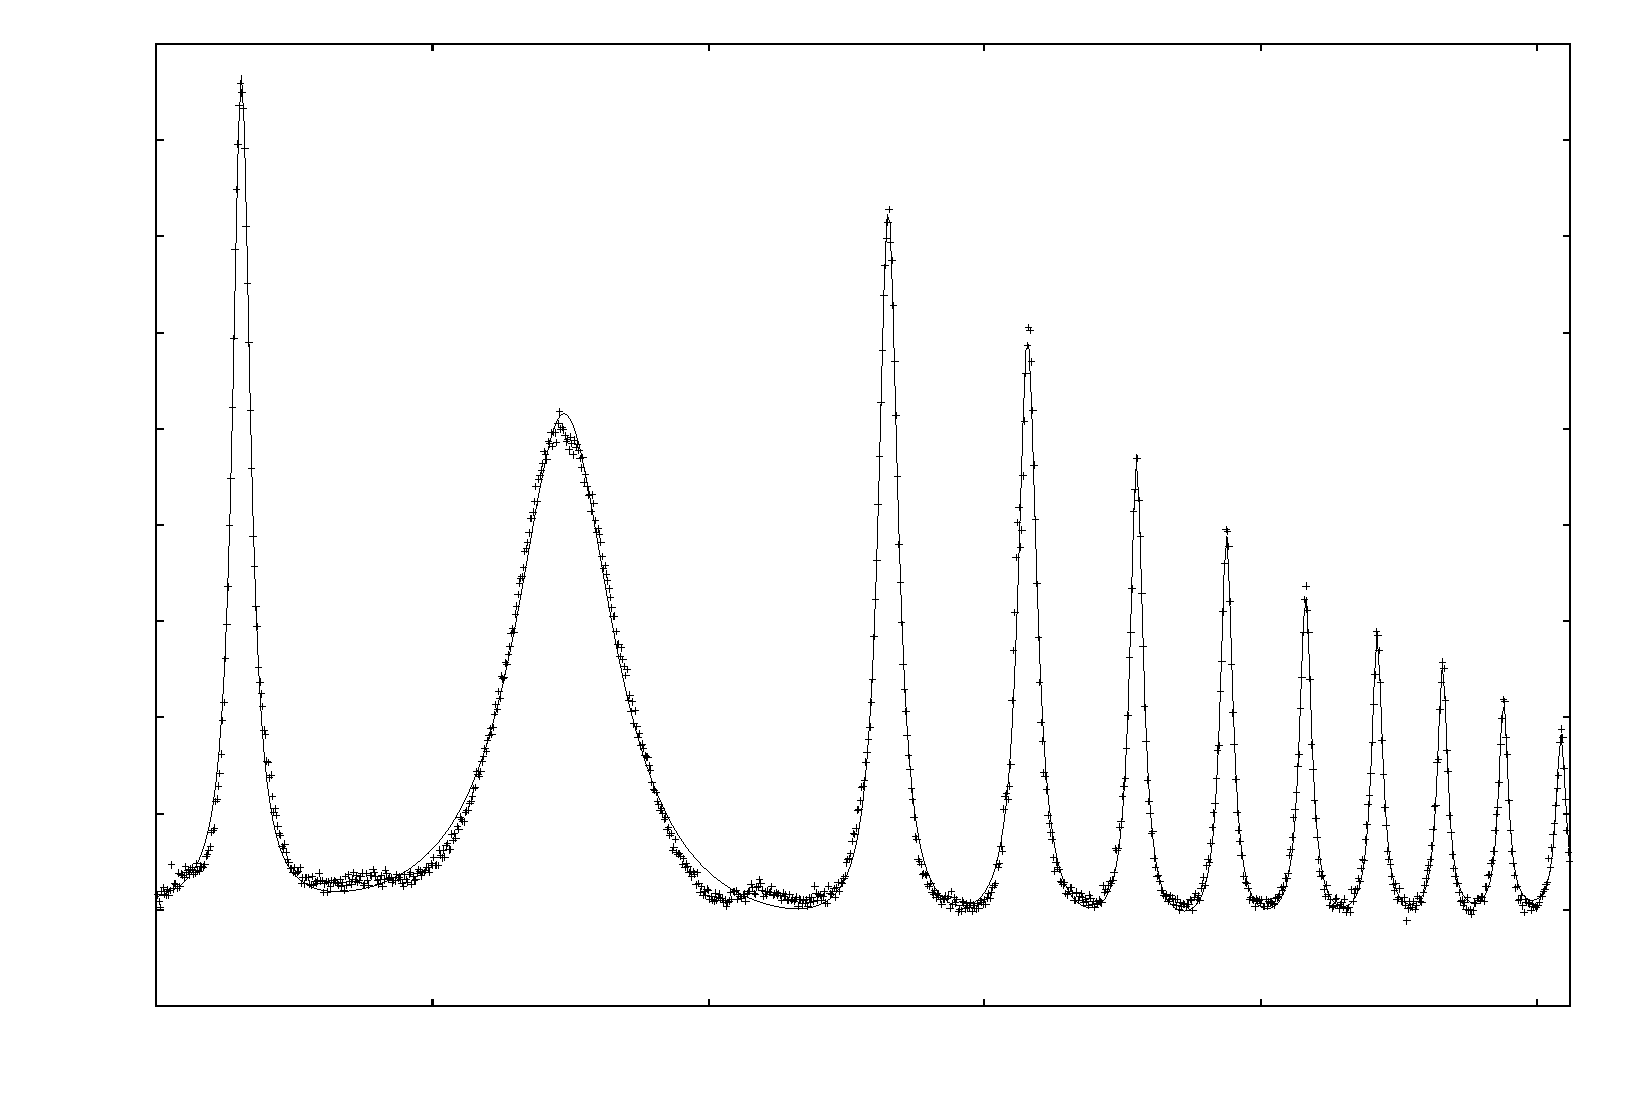
\includegraphics{plot-1}}%
    \gplfronttext
  \end{picture}%
\endgroup

\end{landscape}

\begin{landscape}
  % GNUPLOT: LaTeX picture with Postscript
\begingroup
  \makeatletter
  \providecommand\color[2][]{%
    \GenericError{(gnuplot) \space\space\space\@spaces}{%
      Package color not loaded in conjunction with
      terminal option `colourtext'%
    }{See the gnuplot documentation for explanation.%
    }{Either use 'blacktext' in gnuplot or load the package
      color.sty in LaTeX.}%
    \renewcommand\color[2][]{}%
  }%
  \providecommand\includegraphics[2][]{%
    \GenericError{(gnuplot) \space\space\space\@spaces}{%
      Package graphicx or graphics not loaded%
    }{See the gnuplot documentation for explanation.%
    }{The gnuplot epslatex terminal needs graphicx.sty or graphics.sty.}%
    \renewcommand\includegraphics[2][]{}%
  }%
  \providecommand\rotatebox[2]{#2}%
  \@ifundefined{ifGPcolor}{%
    \newif\ifGPcolor
    \GPcolorfalse
  }{}%
  \@ifundefined{ifGPblacktext}{%
    \newif\ifGPblacktext
    \GPblacktexttrue
  }{}%
  % define a \g@addto@macro without @ in the name:
  \let\gplgaddtomacro\g@addto@macro
  % define empty templates for all commands taking text:
  \gdef\gplbacktext{}%
  \gdef\gplfronttext{}%
  \makeatother
  \ifGPblacktext
    % no textcolor at all
    \def\colorrgb#1{}%
    \def\colorgray#1{}%
  \else
    % gray or color?
    \ifGPcolor
      \def\colorrgb#1{\color[rgb]{#1}}%
      \def\colorgray#1{\color[gray]{#1}}%
      \expandafter\def\csname LTw\endcsname{\color{white}}%
      \expandafter\def\csname LTb\endcsname{\color{black}}%
      \expandafter\def\csname LTa\endcsname{\color{black}}%
      \expandafter\def\csname LT0\endcsname{\color[rgb]{1,0,0}}%
      \expandafter\def\csname LT1\endcsname{\color[rgb]{0,1,0}}%
      \expandafter\def\csname LT2\endcsname{\color[rgb]{0,0,1}}%
      \expandafter\def\csname LT3\endcsname{\color[rgb]{1,0,1}}%
      \expandafter\def\csname LT4\endcsname{\color[rgb]{0,1,1}}%
      \expandafter\def\csname LT5\endcsname{\color[rgb]{1,1,0}}%
      \expandafter\def\csname LT6\endcsname{\color[rgb]{0,0,0}}%
      \expandafter\def\csname LT7\endcsname{\color[rgb]{1,0.3,0}}%
      \expandafter\def\csname LT8\endcsname{\color[rgb]{0.5,0.5,0.5}}%
    \else
      % gray
      \def\colorrgb#1{\color{black}}%
      \def\colorgray#1{\color[gray]{#1}}%
      \expandafter\def\csname LTw\endcsname{\color{white}}%
      \expandafter\def\csname LTb\endcsname{\color{black}}%
      \expandafter\def\csname LTa\endcsname{\color{black}}%
      \expandafter\def\csname LT0\endcsname{\color{black}}%
      \expandafter\def\csname LT1\endcsname{\color{black}}%
      \expandafter\def\csname LT2\endcsname{\color{black}}%
      \expandafter\def\csname LT3\endcsname{\color{black}}%
      \expandafter\def\csname LT4\endcsname{\color{black}}%
      \expandafter\def\csname LT5\endcsname{\color{black}}%
      \expandafter\def\csname LT6\endcsname{\color{black}}%
      \expandafter\def\csname LT7\endcsname{\color{black}}%
      \expandafter\def\csname LT8\endcsname{\color{black}}%
    \fi
  \fi
  \setlength{\unitlength}{0.0500bp}%
  \begin{picture}(15306.00,10204.00)%
    \gplgaddtomacro\gplbacktext{%
      \csname LTb\endcsname%
      \put(1342,704){\makebox(0,0)[r]{\strut{} 0}}%
      \put(1342,1544){\makebox(0,0)[r]{\strut{} 50000}}%
      \put(1342,2383){\makebox(0,0)[r]{\strut{} 100000}}%
      \put(1342,3223){\makebox(0,0)[r]{\strut{} 150000}}%
      \put(1342,4062){\makebox(0,0)[r]{\strut{} 200000}}%
      \put(1342,4902){\makebox(0,0)[r]{\strut{} 250000}}%
      \put(1342,5741){\makebox(0,0)[r]{\strut{} 300000}}%
      \put(1342,6581){\makebox(0,0)[r]{\strut{} 350000}}%
      \put(1342,7420){\makebox(0,0)[r]{\strut{} 400000}}%
      \put(1342,8260){\makebox(0,0)[r]{\strut{} 450000}}%
      \put(1342,9099){\makebox(0,0)[r]{\strut{} 500000}}%
      \put(1342,9939){\makebox(0,0)[r]{\strut{} 550000}}%
      \put(1474,484){\makebox(0,0){\strut{} 1}}%
      \put(3153,484){\makebox(0,0){\strut{} 2}}%
      \put(4833,484){\makebox(0,0){\strut{} 3}}%
      \put(6512,484){\makebox(0,0){\strut{} 4}}%
      \put(8192,484){\makebox(0,0){\strut{} 5}}%
      \put(9871,484){\makebox(0,0){\strut{} 6}}%
      \put(11550,484){\makebox(0,0){\strut{} 7}}%
      \put(13230,484){\makebox(0,0){\strut{} 8}}%
      \put(14909,484){\makebox(0,0){\strut{} 9}}%
      \put(176,5321){\rotatebox{-270}{\makebox(0,0){\strut{}$r_i^2$}}}%
      \put(8191,154){\makebox(0,0){\strut{}Ringindex $i$}}%
      \put(2414,9016){\makebox(0,0)[l]{\strut{}Bestimmung der Brennweite (Aufgabe 5.4)}}%
      \put(2414,8796){\makebox(0,0)[l]{\strut{}Fitgleichung: $A(x) = m x$}}%
      \put(2414,8576){\makebox(0,0)[l]{\strut{}$m = \num{57900.021+-118.118}$}}%
    }%
    \gplgaddtomacro\gplfronttext{%
    }%
    \gplbacktext
    \put(0,0){\includegraphics{plot-2}}%
    \gplfronttext
  \end{picture}%
\endgroup

\end{landscape}


\end{document}
